\chapter{Smart-BMS Software-in-the-Loop Validation}
\label{chap:sil_validation}

\section{Coupling the Physical and Algorithmic Domains}
\label{sec:sil_coupling}

Chapter~10 developed the Simulink-based physical plant model of the battery cell -- a first-order Thevenin ECM parameterized with the offline and online identification methods of Chapters~4 through~9 -- and subjected it to a structured dynamic stress-testing framework spanning idle, partial-load, and high-current excitation. That plant model, on its own, answers only half of the question this report set out to address: it shows how a battery \emph{behaves}, but it says nothing about how accurately a BMS's parameter and state estimation algorithms -- the RLS, EKF, UKF, observer-based, co-estimation, and AI-driven methods developed across Chapters~4 through~9 -- \emph{track} that behavior once it is corrupted by measurement noise, initialized from imperfect starting conditions, and constrained by the limited computational resources of an embedded microcontroller. 

This chapter closes that gap by coupling the physical plant model of Chapter~10 to the algorithmic (estimation) domain in a software-in-the-loop (SIL) simulation environment. By evaluating the resulting closed-loop system against transient tracking and real-time computational criteria, this chapter determines whether a given estimation method is ultimately fit for deployment in a production BMS.

\subsection{Chapter Roadmap}
\label{ssec:ch11_roadmap}

Section~\ref{ssec:xil_taxonomy} places SIL testing within the broader MIL/SIL/PIL/HIL verification hierarchy and Section~\ref{ssec:sil_architecture} develops the specific signal architecture used to couple the Chapter~10 plant model to the algorithmic domain, with Sections~\ref{ssec:sil_nonrealtime}--\ref{ssec:sil_reproducibility} addressing practical considerations: non-real-time execution, test-case coverage, and statistical reproducibility. Section~\ref{sec:transient_tracking} develops the transient-tracking evaluation itself, fixing quantitative metrics (Section~\ref{ssec:transient_metrics}) before applying them to abrupt load-disconnects (Section~\ref{ssec:load_disconnect}) and voltage-estimate stabilization (Section~\ref{ssec:voltage_peak_stabilization}). Section~\ref{sec:realtime_efficiency} shifts from accuracy to computational cost, establishing execution-rate targets, comparing algorithm complexity, and cataloguing embedded implementation-level optimization techniques. Section~\ref{sec:summary_ch11} closes the chapter by synthesizing the accuracy/cost trade-off.

\subsection{Notation Used in This Chapter}
\label{ssec:ch11_notation}

Table~\ref{tab:ch11_notation} collects the symbols introduced specifically in this chapter, extending the notation table first established in Chapter~2.

\begin{table}[htbp]
	\centering
	\caption{Notation introduced in Chapter~11.}
	\label{tab:ch11_notation}
	\renewcommand{\arraystretch}{1.3}
	\begin{tabularx}{\textwidth}{@{}l X l@{}}
		\toprule
		\textbf{Symbol} & \textbf{Meaning} & \textbf{First used} \\
		\midrule
		$\hat{x}(t)$ & Estimated value of a state or parameter $x(t)$ & Eq.~\eqref{eq:rmse} \\
		$\mathrm{RMSE}$ & Root-mean-square error between a true and estimated trajectory & Eq.~\eqref{eq:rmse} \\
		$\hat{V}_t(t)$ & Estimator-internal predicted terminal voltage & Sec.~\ref{ssec:voltage_peak_stabilization} \\
		$N_{\text{trial}}$ & Number of independent SIL trials in a repeated-trial evaluation & Sec.~\ref{ssec:sil_reproducibility} \\
		$n$ & Dimension of the estimated state/parameter vector & Sec.~\ref{ssec:algorithm_complexity} \\
		\bottomrule
	\end{tabularx}
\end{table}

\subsection{Verification and Validation Levels: MIL, SIL, PIL, and HIL}
\label{ssec:xil_taxonomy}

\begin{figure}[htbp]
    \centering
    % Remove the tikzpicture and uncomment the \includegraphics line when you have your image
    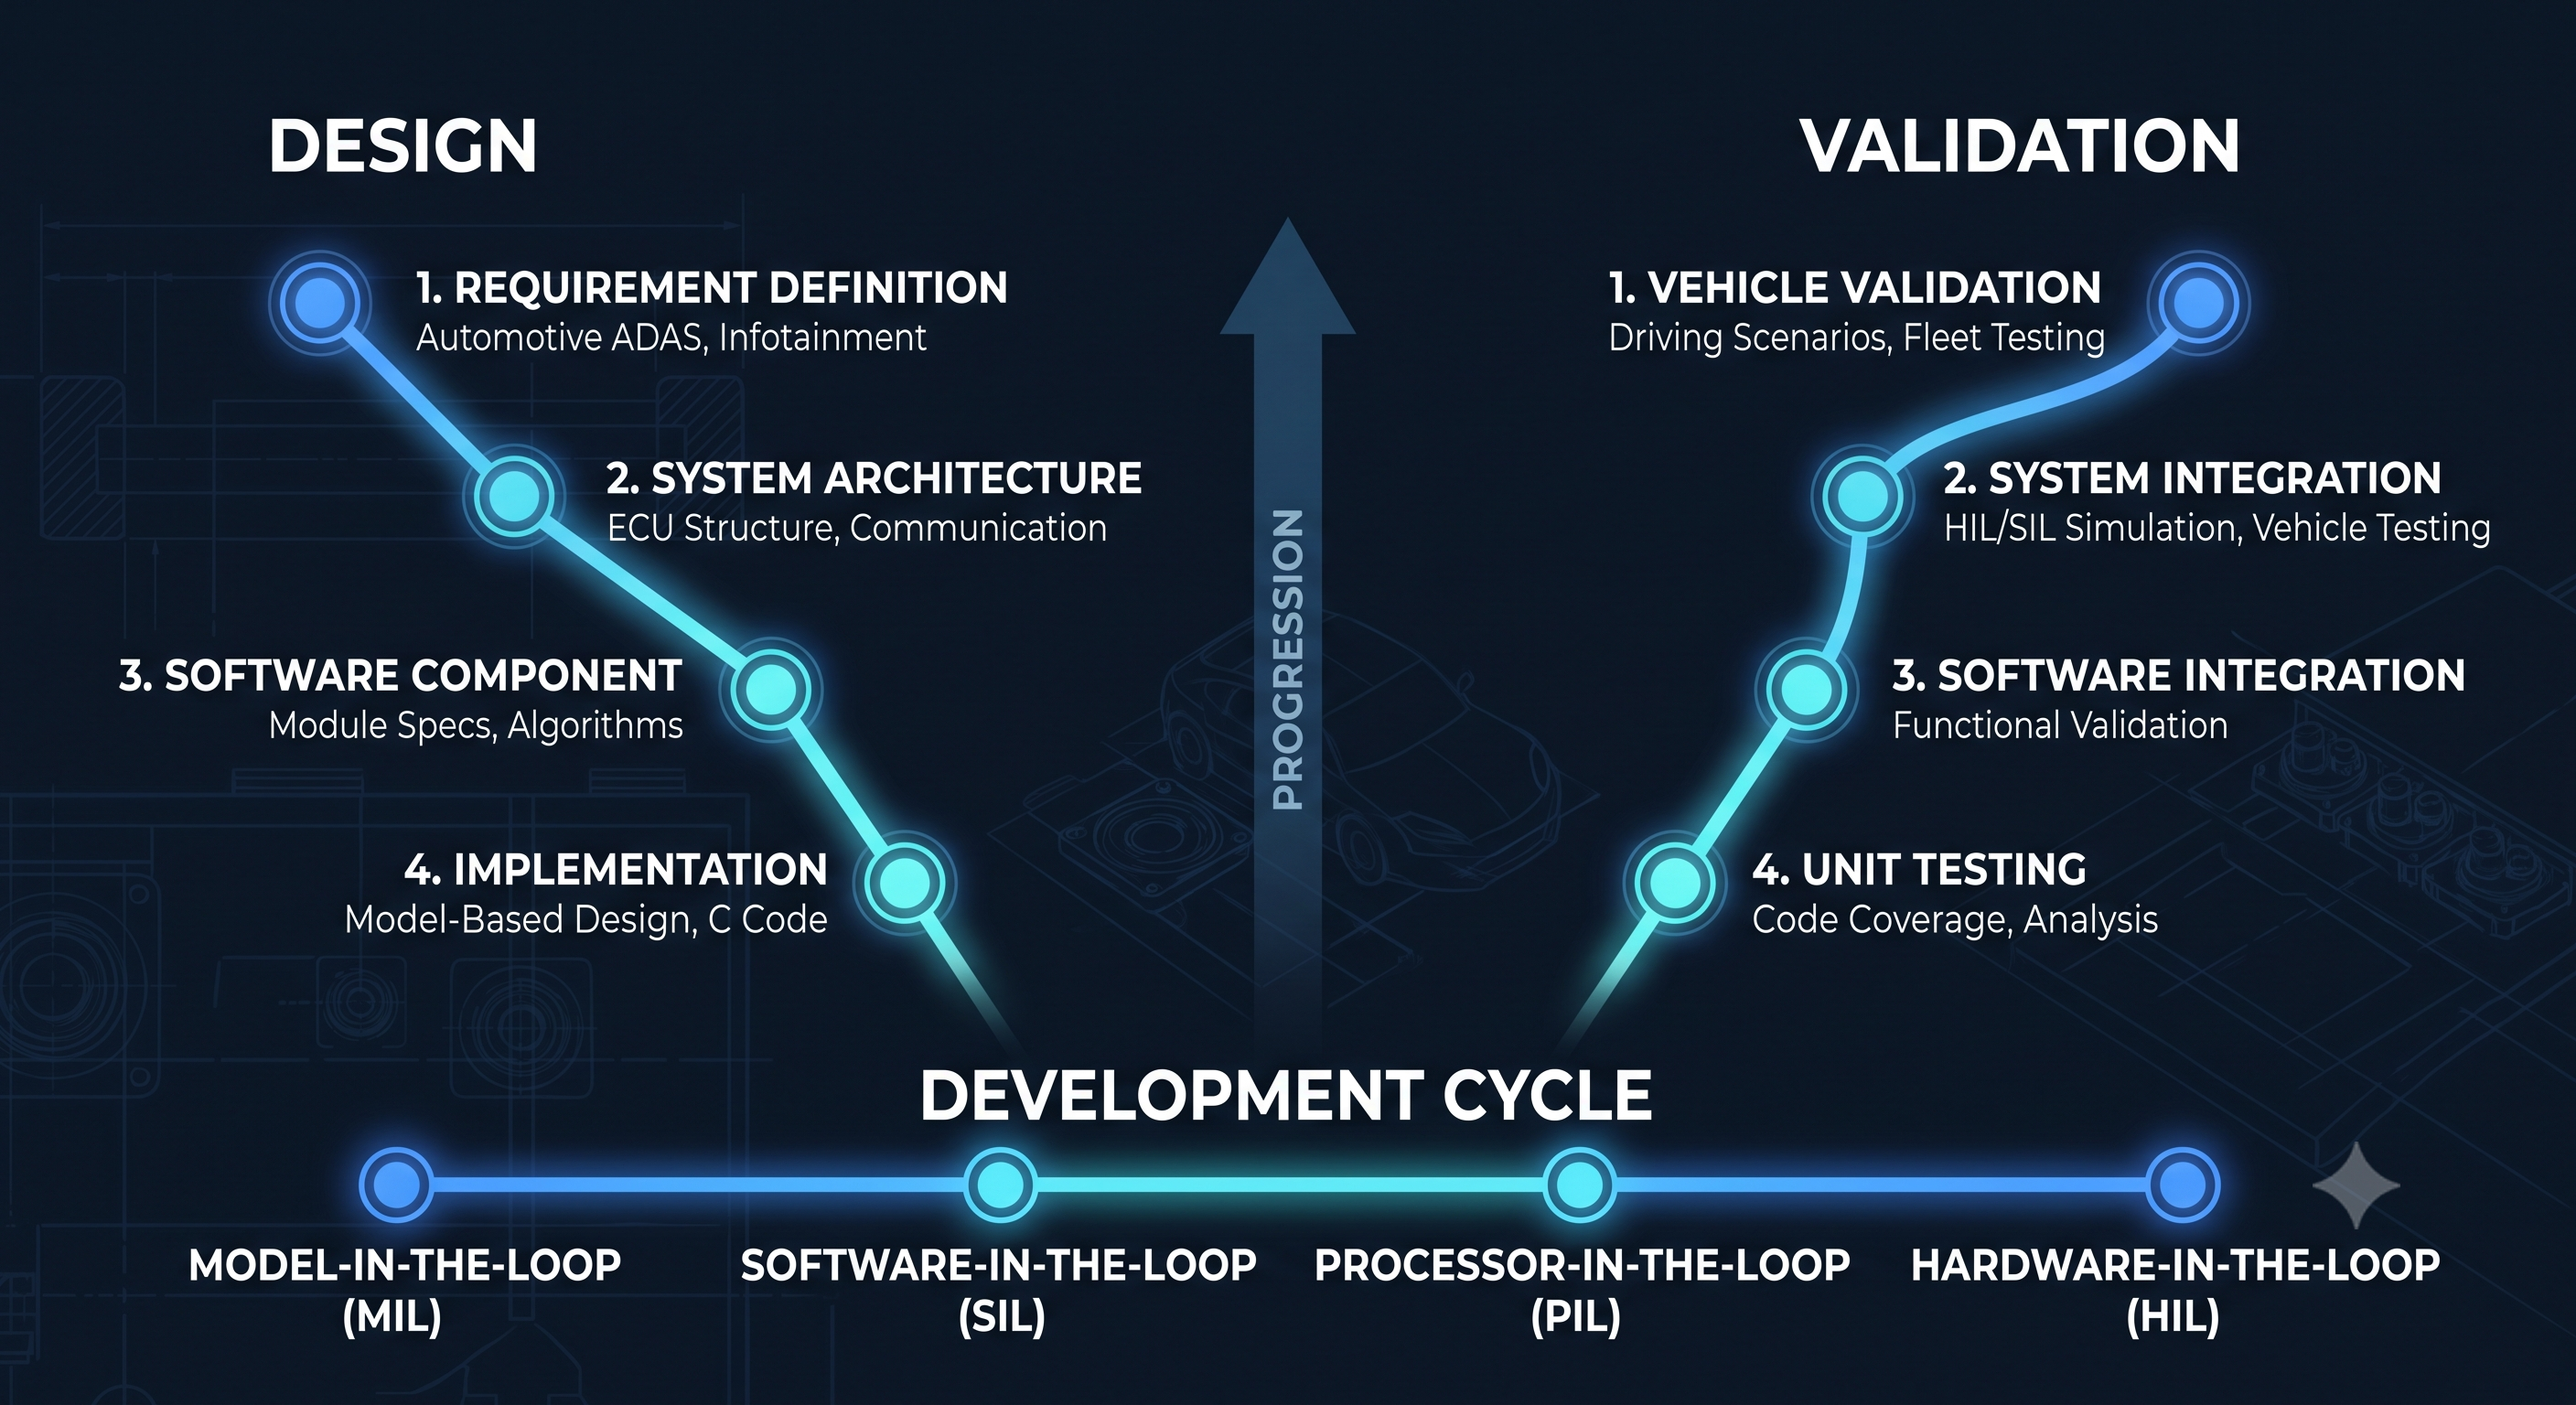
\includegraphics[width=0.85\textwidth]{ch13.png}
    
    \caption{The verification and validation progression from Model-in-the-Loop (MIL) to Hardware-in-the-Loop (HIL).}
    \label{fig:11_xil_hierarchy}
\end{figure}

Before developing the SIL architecture, it is useful to place it within the broader verification and validation (V\&V) hierarchy used in automotive and embedded-systems engineering practice. This hierarchy is commonly organized around four progressively more hardware-realistic stages, mapped onto the right-hand (verification) branch of the V-model of embedded software development \cite{patsnap_hil_sil}:

\begin{itemize}
	\item \textbf{Model-in-the-Loop (MIL).} Both the estimation algorithm and the plant model are executed as high-level Simulink models, with no compiled code and no target hardware involved; computations are performed in floating-point arithmetic.
	\item \textbf{Software-in-the-Loop (SIL).} The estimation algorithm is compiled (or auto-code-generated, in the MathWorks Embedded Coder sense) into the same source-code form that will ultimately run on the BMS microcontroller. This compiled code is executed on a host PC, coupled to the plant model rather than physical hardware.
	\item \textbf{Processor-in-the-Loop (PIL).} The compiled code is moved onto the actual target microcontroller (or an evaluation board), executed in isolation, with its inputs and outputs driven by the plant model running on a host PC. This exposes target-specific numerical behavior (fixed-point rounding, compiler optimization, genuine execution timing).
	\item \textbf{Hardware-in-the-Loop (HIL).} The complete BMS hardware is connected to a real-time simulated battery pack, typically implemented on dedicated real-time target hardware (e.g., Speedgoat) capable of emulating individual cell voltages at update rates of 1~kHz or higher.
\end{itemize}

\begin{table}[htbp]
	\centering
	\caption{Verification and validation levels for BMS estimation algorithms, in order of increasing hardware fidelity.}
	\label{tab:xil_levels}
	\renewcommand{\arraystretch}{1.3}
	\begin{tabularx}{\textwidth}{@{}l X X X@{}}
		\toprule
		\textbf{Level} & \textbf{Estimation algorithm form} & \textbf{Plant model} & \textbf{Primary purpose} \\
		\midrule
		MIL & Simulink model (floating point) & Simulink model & Algorithmic correctness, reference generation \\
		SIL & Compiled/auto-generated code, host PC & Simulink model, host PC & Transient tracking and preliminary timing \\
		PIL & Compiled code, target microcontroller & Simulink model, host PC & Target-specific numerics and execution timing \\
		HIL & Deployed BMS hardware & Real-time target (e.g. Speedgoat) & Full closed-loop, sensor-realistic validation \\
		\bottomrule
	\end{tabularx}
\end{table}

\subsection{SIL Architecture for This Report}
\label{ssec:sil_architecture}

The SIL environment developed in this chapter couples two previously independent halves of this report into a single closed-loop simulation. In modern environments, this coupling is increasingly mediated by the Functional Mock-up Interface (FMI) standard, where the plant model and the BMS code are exported as Functional Mock-up Units (FMUs) to ensure interoperability across different simulation engines.

\begin{enumerate}
	\item \textbf{The physical domain}, consisting of the Chapter~10 Simulink plant model -- the first-order Thevenin ECM parameterized from the offline and online identification results, and exercised under dynamic stress-testing profiles.
	\item \textbf{The algorithmic domain}, consisting of a compiled, deployment-representative implementation of one or more estimation algorithms (e.g., an EKF or sliding-mode observer) that receives the applied current excitation and a noise-corrupted version of the plant's terminal voltage output.
\end{enumerate}

The essential feature distinguishing this SIL coupling is the availability of \emph{ground truth}. Because the plant model's internal states ($z(t)$, $U_p(t)$) and parameters ($R_0$, $R_1$, $C_1$) are accessible signals within the simulation, the estimation algorithm's output can be compared directly against the true simulated quantity at every time step. 

\subsection{Non-Real-Time Execution and Its Implications}
\label{ssec:sil_nonrealtime}

Unlike HIL, where the plant model must execute on dedicated real-time hardware fast enough to keep pace with wall-clock time, a SIL simulation can run faster or slower than real time, limited only by host-PC computational throughput. Because SIL execution time on a host PC bears no fixed relationship to execution time on the target microcontroller, per-step timing measurements taken in SIL are indicative only in a coarse, relative sense. 

\subsection{Test Case Design and Coverage}
\label{ssec:sil_test_design}

The SIL test suite used in this chapter is organized around a small number of current-excitation archetypes:

\begin{itemize}
	\item \textbf{Idle and partial-load transients}, which verify steady-state accuracy.
	\item \textbf{Abrupt load disconnects}, which exercise the fastest dynamics retained in the ECM structures.
	\item \textbf{High-current stress and thermal boundary excitation}, which exercises the estimator's robustness to temperature-dependent parameter drift.
	\item \textbf{Standardized dynamic drive-cycle profiles}, repurposed here as a closed-loop tracking test under application-representative excitation.
\end{itemize}

\subsection{Reproducibility and Statistical Evaluation}
\label{ssec:sil_reproducibility}

Because the measurement noise injected into the SIL loop is a random process, a single SIL run represents only one realization of that noise. Sound SIL evaluation practice therefore repeats each test scenario across multiple independent noise realizations (a Monte Carlo approach) and reports the resulting metric \emph{distributions} (mean and standard deviation) rather than a single-run point value.

\section{Transient Tracking Performance}
\label{sec:transient_tracking}

\subsection{Evaluation Metrics}
\label{ssec:transient_metrics}

\begin{itemize}
	\item \textbf{Root-mean-square error (RMSE).} For an estimate $\hat{x}(t)$ compared against the ground-truth $x(t)$ over a window of $N$ samples:
	\begin{equation}
		\mathrm{RMSE} = \sqrt{\frac{1}{N}\sum_{k=1}^{N} \big(x_k - \hat{x}_k\big)^2}
		\label{eq:rmse}
	\end{equation}
	\item \textbf{Convergence time.} The elapsed time following a transient excitation event required for the estimation error to fall within and remain within a specified tolerance band.
	\item \textbf{Overshoot.} The maximum excursion of an estimate beyond its eventual steady-state value.
	\item \textbf{Estimation error during the transient window.} Evaluated to catch transient-specific error spikes immediately following a step change.
\end{itemize}

\subsection{Response to Abrupt Load Disconnects}
\label{ssec:load_disconnect}

An abrupt load disconnect -- a step change in applied current from a sustained nonzero value to zero -- is among the most demanding transient excitations an estimation algorithm can face. 

\begin{table}[htbp]
	\centering
	\caption{Transient behaviors evaluated under the abrupt load-disconnect scenario, and their traceable causes.}
	\label{tab:load_disconnect_modes}
	\renewcommand{\arraystretch}{1.3}
	\begin{tabularx}{\textwidth}{@{}l X l@{}}
		\toprule
		\textbf{Observed behavior} & \textbf{Likely cause} & \textbf{Report section} \\
		\midrule
		Lagging state estimate & Process-noise covariance mistuned relative to true transient rate. & Ch.~5 \\
		Transient parameter spike & Weak state/parameter distinguishability during sharp excitation. & Ch.~7, Sec.~7.1 \\
		Growing / oscillatory error & ECM order mismatch between estimator and plant, or unstable observer gain. & Ch.~2 \& Ch.~6 \\
		\bottomrule
	\end{tabularx}
\end{table}

\subsection{Dynamic Stabilization of Voltage Peaks}
\label{ssec:voltage_peak_stabilization}

The estimator's predicted terminal voltage, $\hat{V}_t(t)$, can exhibit transient peaks that do not correspond to any physical voltage excursion of the plant. These artifacts stem from:
\begin{enumerate}
	\item \textbf{Excessive Kalman gain:} Immediately following a disconnect, the measurement innovation is large. A large Kalman gain $K_k$ can over-weight this innovation, causing overshoot. 
	\item \textbf{Observer gain selection:} In PI and sliding-mode observers, high switching gains minimize convergence time but increase susceptibility to chattering in the presence of noise.
\end{enumerate}

Given a prior state estimate $\hat{x}_k^-$ and measurement $y_k$, the updated estimate is:
\begin{equation}
	\hat{x}_k = \hat{x}_k^- + K_k \big(y_k - h(\hat{x}_k^-)\big)
	\label{eq:kf_update}
\end{equation}
If $K_k$ is large when the bracketed innovation term is momentarily inaccurate due to a fast step, $\hat{x}_k$ is driven past the true post-transient value. Adaptive innovation-based gain scaling, or boundary-layer smoothing (for sliding-mode observers), are standard mitigations.



\begin{table}[htbp]
	\centering
	\caption{Template for reporting SIL transient-tracking results across repeated Monte Carlo trials.}
	\label{tab:sil_metric_summary_template}
	\renewcommand{\arraystretch}{1.3}
	\begin{tabularx}{\textwidth}{@{}X X c c c@{}}
		\toprule
		\textbf{Scenario} & \textbf{Metric} & \textbf{Mean} & \textbf{Std.\ dev.} & \textbf{Trials} \\
		\midrule
		Load disconnect & SOC convergence time (s) & -- & -- & -- \\
		Load disconnect & Peak transient SOC error (\%) & -- & -- & -- \\
		Load disconnect & Post-transient SOC RMSE (\%) & -- & -- & -- \\
		Load disconnect & $\hat{R}_0$ transient overshoot (m$\Omega$) & -- & -- & -- \\
		High-current stress & SOC RMSE (\%) & -- & -- & -- \\
		Drive-cycle profile & SOC RMSE (\%) & -- & -- & -- \\
		\bottomrule
	\end{tabularx}
\end{table}

\section{Real-Time Computational Efficiency}
\label{sec:realtime_efficiency}

\subsection{Execution Rate Requirements}
\label{ssec:realtime_requirements}
Production BMS estimation algorithms commonly execute at update rates between 100~Hz and 500~Hz. An algorithm whose worst-case execution time exceeds the corresponding sample interval (2--10~ms) cannot be deployed at that rate without algorithmic simplification.

\subsection{Algorithm-Level Computational Complexity}
\label{ssec:algorithm_complexity}

The covariance update step for Kalman-filter-type methods scales cubically with the dimension of the estimated state/parameter vector ($n$):
\begin{equation}
	C_{\text{KF}} = \mathcal{O}(n^3)
	\label{eq:kf_complexity}
\end{equation}
For the UKF, this cost must be evaluated separately for each of the $2n+1$ sigma points, giving an overall per-cycle cost of approximately:
\begin{equation}
	C_{\text{UKF}} \approx (2n+1)\, \mathcal{O}(n^3) = \mathcal{O}(n^4)
	\label{eq:ukf_complexity}
\end{equation}

\begin{table}[htbp]
	\centering
	\caption{Formal per-cycle computational complexity of estimation methods.}
	\label{tab:formal_complexity}
	\renewcommand{\arraystretch}{1.3}
	\begin{tabularx}{\textwidth}{@{}l X l l@{}}
		\toprule
		\textbf{Method} & \textbf{Dominant per-cycle cost} & \textbf{Scaling} & \textbf{Equation} \\
		\midrule
		RLS & Covariance/gain update & $\mathcal{O}(p^2)$ & Sec.~5.1 \\
		EKF & Single-point covariance propagation & $\mathcal{O}(n^3)$ & Eq.~\eqref{eq:kf_complexity} \\
		UKF & $(2n{+}1)$-point covariance propagation & $\mathcal{O}(n^4)$ & Eq.~\eqref{eq:ukf_complexity} \\
		\bottomrule
	\end{tabularx}
\end{table}

\begin{table}[htbp]
	\centering
	\caption{Qualitative and reported comparative computational cost of estimation methods.}
	\label{tab:computational_cost}
	\renewcommand{\arraystretch}{1.3}
	\begin{tabularx}{\textwidth}{@{}l l X l@{}}
		\toprule
		\textbf{Method} & \textbf{Relative cost} & \textbf{Dominant cost driver} & \textbf{Ref.} \\
		\midrule
		RLS (Ch.~5) & Low & Single covariance/gain update per cycle. & Sec.~5.1 \\
		EKF (Ch.~5) & Low--Mod & Single-point Jacobian linearization; scales with ECM order. & Sec.~5.2.1 \\
		UKF (Ch.~5) & Mod--High & $2n+1$ sigma-point propagation per cycle. & Sec.~5.2.2 \\
		Particle filter & High & Scales with particle count. & Sec.~5.3 \\
		Observers & Low & Simple gain-based correction; no covariance propagation. & Sec.~6.2 \\
		GA / PSO & High (offline) & Scales with population size and generation count. & Sec.~4.3 \\
		\bottomrule
	\end{tabularx}
\end{table}

\subsection{Embedded Optimization Techniques}
\label{ssec:embedded_optimization}
To reduce footprint without altering the mathematics:
\begin{itemize}
	\item \textbf{Lookup-table substitution:} Replaces floating-point transcendental function calls.
	\item \textbf{Fixed-point arithmetic:} Manages numerical scaling on hardware without FPUs.
	\item \textbf{Matrix operation restructuring:} Exploits the sparsity or structure of the specific ECM's system matrices (e.g., diagonal structures).
\end{itemize}

\subsection{SIL Test Harness: Algorithmic Summary}
\label{ssec:sil_harness_pseudocode}

\begin{algorithm}[htbp]
\caption{SIL Evaluation of an Estimation Algorithm}
\label{alg:sil_evaluation}
\begin{algorithmic}[1]
\State \textbf{Input:} Plant model, parameter set, estimation algorithm under test, test-scenario profiles, noise model, number of trials $N_{\text{trial}}$.
\State \textbf{Output:} Distribution of transient-tracking metrics and per-cycle execution-time stats.
\For{each test scenario $\in \{\text{idle, load disconnect, thermal, drive-cycle}\}$}
    \For{trial $j = 1 \dots N_{\text{trial}}$}
        \State Draw independent noise realization from measurement-noise model.
        \State Simulate plant under current profile, logging true states $z(t), U_p(t), R_0, R_1, C_1$.
        \State Apply noise realization to terminal voltage to form measured inputs.
        \State Execute compiled estimation algorithm against noisy measurements.
        \State Log estimated states $\hat{z}(t)$, parameters $\hat{R}_0(t)$, and SIL execution time.
        \State Compute trial's RMSE, convergence time, and overshoot metrics.
    \EndFor
    \State Aggregate $N_{\text{trial}}$ trial-level metrics into mean and standard deviation.
\EndFor
\State Compare aggregated metrics across candidate estimation algorithms to inform accuracy vs. cost trade-offs.
\State \textbf{Optional:} Validate target-representative numerics by repeating subset in PIL/HIL.
\end{algorithmic}
\end{algorithm}

\section{Summary}
\label{sec:summary_ch11}

This chapter coupled the physical plant model of Chapter~10 to the algorithmic estimation methods of Chapters~5 through~9 within a software-in-the-loop simulation environment. Transient tracking performance was evaluated using the abrupt load-disconnect scenario, identifying three distinct failure modes. Real-time computational efficiency quantified the cost side of the trade-off. Table~\ref{tab:ch11_consolidated} consolidates these evaluations.

\begin{table}[htbp]
	\centering
	\caption{Consolidated index of Chapter~11 evaluation results by estimation-method family.}
	\label{tab:ch11_consolidated}
	\renewcommand{\arraystretch}{1.3}
	\begin{tabularx}{\textwidth}{@{}l X X l@{}}
		\toprule
		\textbf{Method family} & \textbf{Transient tracking} & \textbf{Real-time cost} & \textbf{Chapter} \\
		\midrule
		RLS / variants & General metrics & Low cost & Ch.~5 \\
		EKF & Load disconnects, voltage peaks & Low--moderate & Ch.~5 \\
		UKF & Load disconnects, voltage peaks & Moderate--high & Ch.~5 \\
		Particle filter & General metrics & High & Ch.~5 \\
		PI / SMO observers & Voltage peak stabilization & Low & Ch.~6 \\
		Co-estimation & Parameter corruption & Scales with $n$ & Ch.~7 \\
		\bottomrule
	\end{tabularx}
\end{table}